\documentclass[12pt]{article}
\usepackage[width=16cm]{geometry}                % See geometry.pdf to learn the layout options. There are lots.
\geometry{letterpaper}                   % ... or a4paper or a5paper or ... 
%\geometry{landscape}                % Activate for for rotated page geometry
%\usepackage[parfill]{parskip}    % Activate to begin paragraphs with an empty line rather than an indent
\usepackage{graphicx}
\usepackage{amssymb}
\usepackage{amsmath}
\usepackage{aliases}
\usepackage{color}

\usepackage{listings}
\usepackage{cancel}
\usepackage{textcomp}

\lstset{
   language=matlab,
   keywordstyle=\bfseries\ttfamily\color[rgb]{0,0,1},
   identifierstyle=\ttfamily,
   commentstyle=\color[rgb]{0.133,0.545,0.133},
   stringstyle=\ttfamily\color[rgb]{0.627,0.126,0.941},
   showstringspaces=false,
   basicstyle=\small,
   numberstyle=\footnotesize,
   numbers=none,
   stepnumber=1,
   numbersep=10pt,
   tabsize=2,
   breaklines=true,
   prebreak = \raisebox{0ex}[0ex][0ex]{\ensuremath{\hookleftarrow}},
   breakatwhitespace=false,
   aboveskip={0.1\baselineskip},
    columns=fixed,
    upquote=true,
    extendedchars=true,
% frame=single,
    backgroundcolor=\color[rgb]{0.9,0.9,0.9}
}

\title{Two dimensional heat equation}
\author{Praveen. C, Deep Ray, Jean-Pierre Raymond}
%\date{}                                           % Activate to display a given date or no date

\begin{document}



\maketitle
%\section{}
%\subsection{}


\section{The model}
Let $z = z(x,y,t)$ denote the temperature. 
The shifted 2-D heat equation is given by
\[
z_t = \mu \Delta z + \alpha z, \quad (x,y) \in \Omega = (0,1) \times (0,1), \qquad t \in  [0,T]
\]
with boundary conditions
\[
z(x,0,t) = z(x,1,t) = 0, \quad z(1,y,t) = u(y,t), \qquad \df{z}{x}(0,y,t) = 0
\]
and initial condition
\[
z(x,y,0) = z_0(x,y)
\]
Here $\alpha \ge 0$ and $\mu > 0$. Let us denote the Dirichlet part of the boundary by $\Gamma_D$
\[
\Gamma_D = \{ y=0\} \cup \{ y=1\} \cup \{ x=1 \}
\]
the Neumann part as
\[
\Gamma_N = \{ x=0 \}
\]
and the part on which the control is applied as
\[
\Gamma_c = \{ x=1 \}
\]
\begin{figure}
\begin{center}
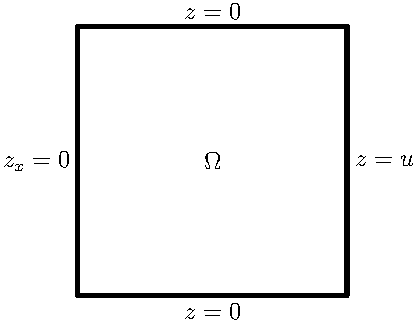
\includegraphics[width=0.5\textwidth]{heat2d_prob}
\caption{Problem definition}
\end{center}
\end{figure}
%------------------------------------------------------------------------------

\subsection{Observations}
We will measure an average value of the temperature on strips along the left vertical boundary
\[
I_i = [a_i, b_i]
\]
as shown in figure. Thus the observations are
\begin{equation}
y_i(t) = \frac{1}{b_i - a_i} \int_{a_i}^{b_i} z(0,y,t) \ud y
\end{equation}

\begin{figure}
\begin{center}
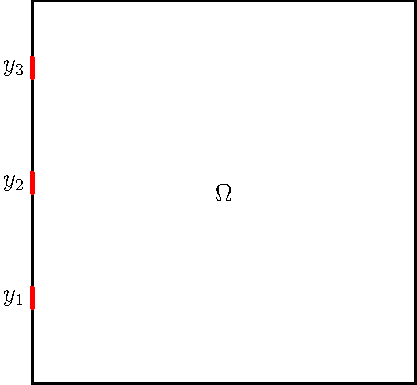
\includegraphics[width=0.5\textwidth]{heat2d_obs}
\caption{Observations}
\end{center}
\end{figure}
%------------------------------------------------------------------------------
\subsection{Weak formulation}
We assume $z_0 \in L^2(\Omega)$. We wish to find $z \in L^2(0,T;H^1(\Omega))$ such that
\[
 \dd{}{t}(z(t), \phi)_{L^2} = - \mu \int_\Omega \nabla z \cdot \nabla \phi \ud x +  \alpha \int_\Omega z \phi \ud x, \quad \forall \phi \in H^1_{\Gamma_D}(\Omega)
\]
\[
z(x,0,t) = z(x,1,t) = 0, \quad z(1,y,t) = u(y,t)
\]
\[
 (z(0),\phi)_{L^2} = (z_0 ,\phi)_{L^2}
\]
%------------------------------------------------------------------------------

\section{FEM approximation}
\begin{figure}
\begin{center}
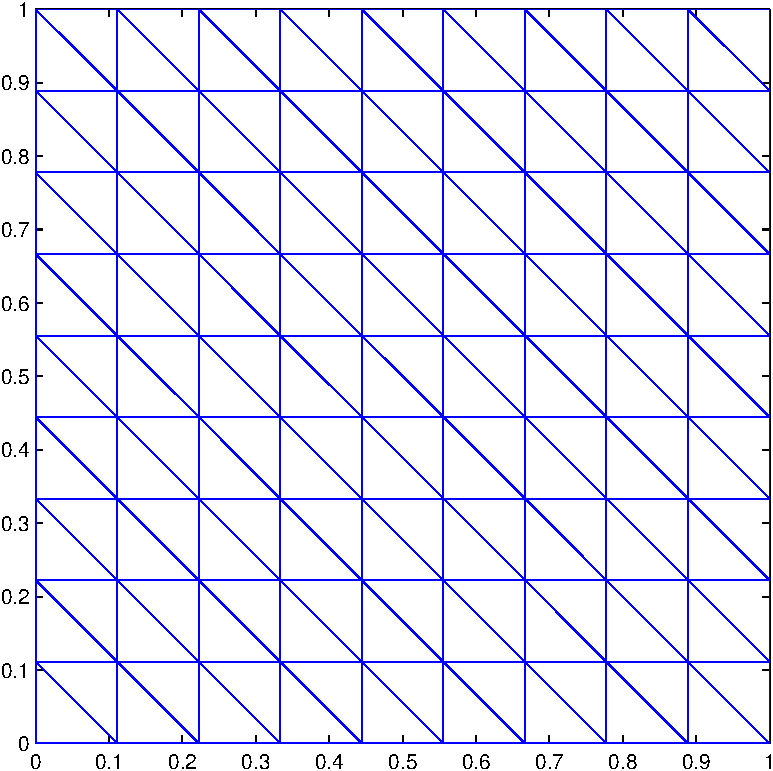
\includegraphics[width=0.5\textwidth]{heat2d_mesh}
\caption{Example of a finite element mesh}
\end{center}
\end{figure}
Consider a division of $\Omega$ into disjoint triangles as shown in figure~(xxx). We will assume that the vertices of the mesh are numbered in some manner. Let us define the following sets of vertices
\begin{eqnarray*}
N_c &=& \mbox{vertices on $\Gamma_c$} \\
N_d &=& \mbox{vertices on } \{y=0\} \cup \{y=1\} \\
N_f &=& \mbox{remaining vertices}
\end{eqnarray*}
For each vertex $i$, define the piecewise affine functions $\phi_i(x,y)$ with the property that
\[
\phi_i(x_j, y_j) = \delta_{ij}
\]
We will take the control to be of the form
\[
u(y,t) = v(t) \sin(\pi y)
\]
Then the finite element solution is of the form
\[
z(x,y,t) = \sum_{j \in N_f} z_j(t) \phi_j(x,y) + v(t) \sum_{j \in N_c} \sin(\pi y_j) \phi_j(x,y)
\]
The approximate weak formulation is given as
\[
 \dd{}{t}(z(t), \phi_i)_{L^2} = - \mu \int_\Omega \nabla z \cdot \nabla \phi_i \ud x +  \alpha \int_\Omega z \phi_i \ud x, \quad \forall i \in N_f
\]
i.e.,
\begin{eqnarray*}
&& \sum_{j \in N_f} \dd{z_j}{t} \int_\Omega \phi_j \phi_i + \dd{v}{t} \sum_{j \in N_c} \sin(\pi y_j) \int_\Omega \phi_j \phi_i \\
&=& -\mu \sum_{j \in N_f} z_j \int_\Omega \nabla \phi_j \cdot \nabla \phi_i - \mu v \sum_{j \in N_c} \sin(\pi y_j) \int_\Omega \nabla \phi_j \cdot \nabla \phi_i \\
&& + \alpha \sum_{j \in N_f} z_j \int_\Omega \phi_j \phi_i + \alpha v \sum_{j \in N_c} \sin(\pi y_j) \int_\Omega \phi_j \phi_i, \qquad \forall i \in N_f
\end{eqnarray*}
In order to simplify the presentation we will ignore the term containing $\dd{v}{t}$\footnote{This term vanishes if we use the trapezoidal rule for integration.} and then we can write the FEM formulation as
\begin{eqnarray*}
&& \sum_{j \in N_f} \dd{z_j}{t} \int_\Omega \phi_j \phi_i \\
&=&  \sum_{j \in N_f} z_j \left[ -\mu\int_\Omega \nabla \phi_j \cdot \nabla \phi_i + \alpha \int_\Omega \phi_j \phi_i \right] \\
&& v \sum_{j \in N_c} \left[ - \mu  \sin(\pi y_j) \int_\Omega \nabla \phi_j \cdot \nabla \phi_i + \alpha\sin(\pi y_j) \int_\Omega \phi_j \phi_i \right] \qquad \forall i \in N_f
\end{eqnarray*}
This can be written as a system of differential equations
\[
 \M \dd{\z}{t} = \A \z + \B v
\]

%-----------------------------------------------------------------
\subsection{Finite element assembly}
The finite element basis functions have compact support. Hence we can compute the integrals by adding the contributions from a small number of triangles. For example, the elements of the mass matrix can be computed as
\[
\int_\Omega \phi_i \phi_j = \sum_{K \ : \ i, j \in K} \int_K \phi_i \phi_j
\]
and similarly the stiffness matrix is computed as
\[
\int_\Omega \nabla \phi_i \cdot \nabla \phi_j = \sum_{K \ : \ i, j \in K} \int_K \nabla \phi_i \cdot \nabla \phi_j
\]
The integrals on each triangle $K$ will be evaluated exactly. For a triangle $K$ with vertices labelled 1, 2, 3, the local mass and stiffness matrices are given by
\[
M_K =
\]
%-----------------------------------------------------------------
\subsection{Computing the observation}
%-----------------------------------------------------------------

\end{document}  